\documentclass[compress,noamsthm,hyperref={bookmarksopen=true},aspectratio=169]{beamer}
%\usepackage[bookmarksopen=true]{hyperref}

%---------------------------
% something I add to the preface
\usepackage{graphicx}
\graphicspath{ {./slides-pics/} }
\usepackage{multirow}
\usepackage{verbatim}
\usepackage{color}
\usepackage{rotating}
\newcommand{\hilight}[1]{\colorbox{yellow}{#1}}
%---------------------------


% ----------------------------------------------------------------------
% Packages

% ----------------------------------------------------------------------
% Packages

\usepackage{amsmath,amsthm,amssymb}

\usepackage{tikz}
\usetikzlibrary{calc, positioning, arrows}

\usepackage{hyperref}
\hypersetup{pdfencoding=unicode}

\usepackage{stmaryrd}
\usetikzlibrary{cd}
\usepackage[all,cmtip]{xypic}
\CompileMatrices

\usepackage{kbordermatrix}

% ----------------------------------------------------------------------
% For the bibliography

\newcommand{\arxiv}[1]{arXiv:\urlalt{https://arxiv.org/abs/#1}{#1}}

% ----------------------------------------------------------------------
% Theorem like environments

\theoremstyle{plain}
\newtheorem{theorem}{Theorem}[section]
\newtheorem{lemma}[theorem]{Lemma}
\newtheorem{corollary}[theorem]{Corollary}

\theoremstyle{definition}
\newtheorem{definition}[theorem]{Definition}
\newtheorem{remark}[theorem]{Remark}
\newtheorem{algorithm}[theorem]{Algorithm}

%----------------------------------------------------------------------
% A hack: \m is similar to \vcenter, but works better.
% \mp{0.2}{x}: raise the box x so that 20% of it is below the
% centerline. Unlike \vcenter, don't change the horizontal spacing

\newlength{\localh}
\newlength{\locald}
\newbox\mybox
\def\mp#1#2{\scalebox{0.8}{\setbox\mybox\hbox{#2}\localh\ht\mybox\locald\dp\mybox\addtolength{\localh}{-\locald}\raisebox{-#1\localh}{\box\mybox}}}
\def\m#1{\mp{0.4}{#1}}

%----------------------------------------------------------------------
% Ad hoc quantum circuits using TikZ

\newenvironment{qcircuit}{%
  \begingroup%
  \def\dot##1{\fill (##1) circle (.15);}%
  \def\whitedot##1{\filldraw[fill=white,thick] (##1) circle (.15);}%
  \def\triangle##1{\fill (##1)+(.3,0) --
    +(-.15,.25) -- +(-.15,-.25) -- cycle;}%
  \def\triangleadj##1{\fill (##1)+(-.3,0) --
    +(.15,.25) -- +(.15,-.25) -- cycle;}%
  \def\notgate##1{\filldraw[fill=white,thick] (##1) circle (.3);
                  \draw[thick] (##1)+(.3,0) -- +(-.3,0);
                  \draw[thick] (##1)+(0,.3) -- +(0,-.3);
                }%
  \def\dotgate{\dot}%
  \def\sepgate##1##2##3{
    \fill[fill=white] (##1-.05,##2-.4) rectangle (##1+.05,##2+.4);
    \fill[fill=white] (##1-.05,##3-.4) rectangle (##1+.05,##3+.4);
    \draw[thick, dashed] (##1,##2-.25) -- (##1,##3+.25);
  }%
  \def\swapgate##1##2##3{
    \fill[fill=white] (##1-.45,##2-.4) rectangle (##1+.45,##2+.4);
    \fill[fill=white] (##1-.45,##3-.4) rectangle (##1+.45,##3+.4);
    \draw[thick] (##1-.45,##2) -- (##1+.45,##3);
    \draw[thick] (##1-.45,##3) -- (##1+.45,##2);
  }%
  \def\controlledS##1##2{\controlled{\dotgate}{##1}{##2};%
    \path(##1) node[above right]{$i$}}%              
  \def\controlledSS##1##2{\controlled{\gate{$S$}}{##1}{##2}}%
  \def\controlledSSd##1##2{\controlled{\gate{$S^{\dagger}$}}{##1}{##2}}%
  \def\controlled{\gencontrolled{\dot}}%
  \def\whitecontrolled{\gencontrolled{\whitedot}}%
  \def\controlwires##1##2{\foreach\x in {##2} {
                    \draw[thick] (##1 |- 0,\x) -- (##1);
                  }}%
  \def\gencontrolled##1##2##3##4{\controlwires{##3}{##4};
                  ##2{##3};
                  \foreach\x in {##4} {
                    ##1{##3 |- 0,\x};
                  }}%
  \def\gate##1##2{\biggate{##1}{##2}{##2}}%
  \def\colgate##1##2##3{\widebigcolgate{##2}{##3}{##3}{.45}{##1}}%
  \def\colbiggate##1##2##3##4{\widebigcolgate{##2}{##3}{##4}{.45}{##1}}%
  \def\biggate##1##2##3{\widebiggate{##1}{##2}{##3}{.45}}%
  \def\widegate##1##2##3{\widebiggate{##1}{##3}{##3}{##2}}%
  \def\widebiggate##1##2##3##4{\widebigcolgate{##1}{##2}{##3}{##4}{white}}%
  \def\widecolgate##1##2##3##4{\widebigcolgate{##3}{##4}{##4}{##1}{##2}}%
  \def\widebigcolgate##1##2##3##4##5{\filldraw[fill=##5,thick] (##2)+(-1*##4,-.4)
    rectangle ($(##3)+(##4,.4)$); \draw ($.5*(##2)+.5*(##3)$) node
    {\small ##1};}%
  \def\invisiblewidebigcolgate##1##2##3{\path (##1)+(-1*##3,-.4)
    rectangle ($(##2)+(##3,.4)$);}%
  \def\invisiblegate##1{\invisiblewidebigcolgate{##1}{##1}{.45}}
  \def\gridx##1##2##3{\foreach\x in {##3} {
        \draw[thick] (##1,\x) -- (##2,\x);
      }}%
  \def\grid{\gridx{0}}%
  \def\cross##1{\draw (##1)+(-.3,-.3) -- +(.3,.3);
             \draw (##1)+(.3,-.3) -- +(-.3,.3);}%
  \def\bar##1{\fill (##1)+(-.05,-.4) rectangle ($(##1)+(.05,.4)$);}%
  \def\init##1##2{\bar{##2}; \leftlabel{##1}{##2};}%
  \def\term##1##2{\bar{##2}; \rightlabel{##1}{##2};}%
  \def\leftlabel##1##2{\draw (##2) node[left] {##1};}%
  \def\rightlabel##1##2{\draw (##2) node[right] {##1};}%
  \def\wirelabel##1##2{\draw (##2)+(0,-.15) node[above] {\footnotesize ##1};}%
  \def\multiwire##1{\draw (##1)+(-.1,-.3) -- +(.1,.3);}%
  \begin{tikzpicture}}
  {\end{tikzpicture}\endgroup}

%----------------------------------------------------------------------
% Alphabetic labels

{\makeatletter
\gdef\alphalabels{\def\theenumi{\@alph\c@enumi}\def\labelenumi{(\theenumi)}}}

% ----------------------------------------------------------------------
% Miscellaneous macros

\newcommand{\xmatrix}[4]{{\renewcommand{\arraystretch}{#1}\arraycolsep=#2ex\left(\begin{array}{#3}#4\end{array}\right)}}       % resizable matrix
\newcommand{\zmatrix}{\xmatrix{.8}{.8}}         % matrix
\newcommand{\smatrix}[1]{\begin{bmatrix} #1 \end{bmatrix}}         % matrix
\newcommand{\s}[1]{\left\{#1\right\}}
\newcommand{\cC}{{\cal C}}
\newcommand{\cT}{{\cal T}}
\newcommand{\cCS}{{\mathcal{CCS}}}
\newcommand{\Clifford}{\cC}
\newcommand{\CliffordCS}{\cCS}
\newcommand{\inv}{^{-1}}
\newcommand{\da}{^{\dagger}}
\newcommand{\CZ}{C\kern-.16667em Z}
\newcommand{\CX}{C\kern-.16667em X}
\newcommand{\CS}{C\kern-.16667em S}
\newcommand{\CK}{C\kern-.16667em K}
\newcommand{\XC}{X\kern-.16667em C}
\newcommand{\KC}{K\kern-.16667em C}
\newcommand{\Ex}{E\kern-.16667em x}
\newcommand{\LS}{L\kern-.16667em S}
\newcommand{\RS}{R\kern-.16667em S}
\newcommand{\CCZ}{CCZ}
\newcommand{\CCX}{CCX}
\newcommand{\CCK}{CCK'}
\newcommand{\Swap}{\textit{Swap}}
\newcommand{\CCS}{Clifford+$\CS$ }
\newcommand{\pres}[2]{\langle #1\mid #2 \rangle}


\newcommand{\Xx}{\mathcal{X}}
\newcommand{\Yy}{\mathcal{Y}}
\newcommand{\Rr}{\Delta}
\newcommand{\Ss}{\Gamma}
\newcommand{\Ee}{\mathcal{E}}

\newcommand{\Z}{\mathbb{Z}}
\newcommand{\jay}{j}
\newcommand{\kay}{k}
\newcommand{\tee}{t}
\newcommand{\svdots}{\scalebox{.55}{$\vdots$}}
\newcommand{\seq}{\subseteq}
\newcommand{\gen}[1]{\langle#1\rangle}
\newcommand{\sem}[1]{[#1]}
\newcommand{\semG}[1]{\sem{#1}_{G}}
\newcommand{\semH}[1]{\sem{#1}_{H}}
\newcommand{\simE}{\sim_{\Ee}}
\newcommand{\simR}{\sim_{\Rr}}
\newcommand{\simS}{\sim_{\Ss}}
\newcommand{\Ys}{Y_{s}}
\newcommand{\Rsyll}[1]{R_{#1}}
\newcommand{\ket}[1]{|#1\rangle}

\newcommand{\fst}[1]{\text{fst}(#1)}
\newcommand{\snd}[1]{\text{snd}(#1)}
\newcommand{\Zhi}{\Z[\frac{1}{2},i]}



\newcommand{\Mod}[1]{\,(\mathrm{mod}\ #1)}

\newcommand{\zi}{\Z [i]}
\newcommand{\di}{\D [i]}
\newcommand{\simr}{\sim_{\Rr}}
\newcommand{\oh}{K}
\newcommand{\lde}[1]{\text{lde}( #1 )}
\newcommand{\ldeg}[1]{\text{lde}_{\gamma}( #1 )}

\newcommand{\eqmo}{\equiv_{\gamma}}
\newcommand{\eqmt}{\equiv_{\gamma^2}}
\newcommand{\eqmth}{\equiv_{\gamma^3}}


\newcommand{\level}[1]{\text{level}(#1)}
\newcommand{\xal}{X_{[\alpha, \alpha+1]}}
\newcommand{\normalword}{\text{\rm normal}}
\newcommand{\nf}{\text{\sc nf}}

\newcommand{\tlx}[2]{X_{[#1, #2]}}
\newcommand{\tlkd}[2]{\oh^{\dagger}_{[#1, #2]}}
\newcommand{\tlk}[2]{\oh_{[#1, #2]}}
\newcommand{\tli}[2]{i_{[#1]}^{#2}}

\newcommand{\D}{{\mathbb D}}
\newcommand{\N}{{\mathbb N}}
\newcommand{\R}{{\mathbb R}}
\newcommand{\C}{{\mathbb C}}
\newcommand{\Gg}{\mathcal{G}}
\newcommand{\iso}{\cong}

\newcommand{\sfrac}[2]{{#1}/{#2}}   % short fraction
\newcommand{\norm}[1]{\|#1\|}


\newcommand{\eps}{\varepsilon}


\makeatletter
\newcommand{\xRightarrow}[2][]{\ext@arrow 0359\Rightarrowfill@{#1}{#2}}
\makeatother




% ----------------------------------------------------------------------
% Macros for large case distinctions

% \newcounter{case}
% \newcounter{subcase}[case]
% \newcounter{subsubcase}[subcase]
% \newcounter{subsubsubcase}[subsubcase]
% \newcounter{subsubsubsubcase}[subsubsubcase]

% \renewcommand{\thesubcase}{\thecase.\arabic{subcase}}
% \renewcommand{\thesubsubcase}{\thesubcase.\arabic{subsubcase}}
% \renewcommand{\thesubsubsubcase}{\thesubsubcase.\arabic{subsubsubcase}}
% \renewcommand{\thesubsubsubsubcase}{\thesubsubsubcase.\arabic{subsubsubsubcase}}

% \newcommand{\case}[1]{\refstepcounter{case}\par\noindent{\bf Case \thecase.} #1.}
% \newcommand{\subcase}[1]{\refstepcounter{subcase}\par\noindent{\bf Case \thesubcase.} #1.}
% \newcommand{\subsubcase}[1]{\refstepcounter{subsubcase}\par\noindent{\bf Case \thesubsubcase.} #1.}
% \newcommand{\subsubsubcase}[1]{\refstepcounter{subsubsubcase}\par\noindent{\bf Case \thesubsubsubcase.} #1.}
% \newcommand{\subsubsubsubcase}[1]{\refstepcounter{subsubsubsubcase}\par\noindent{\bf Case \thesubsubsubsubcase.} #1.}




\newcommand{\CliffordT}{\cC\cT}




\newcommand{\De}{\Delta}
\newcommand{\amal}{*}



%\newcommand{\sem}[1]{[#1]}

% Make sure this command does the same thing whether we use pdflatex
% or latex. The problem is that the \urlalt provided in some package
% (perhaps breakurl?) is different that the one provided by eptcs.
\providecommand{\urlalt}[2]{\href{#1}{#2}}
\renewcommand{\urlalt}[2]{\href{#1}{#2}}

\DeclareMathOperator{\rcs}{rcs}
\DeclareMathOperator{\cs}{cs}
\DeclareMathOperator{\kc}{kc}
\DeclareMathOperator{\rkc}{rkc}
\DeclareMathOperator{\rlen}{rlen}
\DeclareMathOperator{\len}{len}
\DeclareMathOperator{\pat}{pat}




\title{Generators and relations for some classes of quantum circuits}

\author{Xiaoning Bian}

\date{Department of Mathematics and Statistics\\
  Dalhousie University}
\begin{document}

\beamertemplatenavigationsymbolsempty

\begin{frame} % Cover slide
  \titlepage
  \begin{center}
    Ph.D. thesis defense, Aug 24, 2023
  \end{center}
\end{frame}


\section*{Outline}
\begin{frame}
\frametitle{Contents}
\tableofcontents
\end{frame}

\section{Introduction}
\subsection{Motivation}
\begin{frame}{Motivation}
  \begin{itemize}\setlength\itemsep{1.2em}
  \item For certain problems such as factoring, quantum algorithms
    give an exponential speedup over the best know classical
    algorithms \cite{Shor}.
  \item For this reason, quantum computing has been a very active area
    of research. Many quantum algorithms use \emph{quantum circuits}
    as building blocks.
  \item This thesis contributes to the theory of quantum circuits.
  \end{itemize}
\end{frame}


\subsection{Clifford, Clifford+$T$, and Clifford+$\CS$ operators}
\begin{frame}{Clifford, Clifford+$T$ and Clifford+$\CS$ operators}
The class of Clifford operators is generated by tensor product and
composition of the following operators:
\[ S =  \begin{bmatrix}
    1 & 0 \\
    0 & i
  \end{bmatrix},
  \, H =  \frac{1}{\sqrt 2}\begin{bmatrix}
    1 & 1 \\
    1 & -1
  \end{bmatrix},
  \, \omega = e^{\frac{\pi}{4}i}=\frac{1+i}{\sqrt 2},
  \, \CZ = \begin{bmatrix}
    1 & 0 & 0 & 0 \\
    0 & 1 & 0 & 0 \\
    0 & 0 & 1 & 0 \\
    0 & 0 & 0 & -1 
  \end{bmatrix}.
\]
Here $S$ is called the \emph{phase gate}, $H$ is called the Hadamard
gate, $\omega$ is a scalar that is an $8$-th root of unity, and $\CZ$
is the controlled $Z$-gate. The class of Clifford+$T$ operators is
generated by the Clifford operators plus the following $T$-gate:
\[ T =  \begin{bmatrix}
    1 & 0 \\
    0 & \omega
  \end{bmatrix}.
\]

\end{frame}

\begin{frame}{Clifford, Clifford+$T$ and Clifford+$\CS$ operators}
  The class of Clifford+$\CS$ operators is generated by the Clifford
  operators plus the controlled $S$-gate:
\[
    \CS = \begin{bmatrix}
    1 & 0 & 0 & 0 \\
    0 & 1 & 0 & 0 \\
    0 & 0 & 1 & 0 \\
    0 & 0 & 0 & i 
  \end{bmatrix}.
\]
Note that $\CZ=\CS^2$. We also use the following gate:
\[
K = \omega\da H = \frac{1}{1+i}\begin{bmatrix}
    1 & 1 \\
    1 & -1
  \end{bmatrix}.
\]
Here $i$ is the complex unit, and $K$ is a scaled version of $H$.

\end{frame}

\begin{frame}{Indexed notation}
Let $I$ be the $2\times 2$ identity operator. We write
\[
  K_0=K\otimes I\otimes I \ldots,\quad K_1=I\otimes K\otimes I \ldots,\quad K_2=I\otimes I\otimes K \otimes I \ldots, \quad \ldots
\]
and similarly for $S_0,S_1, \ldots$ and $H_0,H_1, \ldots$. We write
\[
  \CS_{01}=\CS\otimes I \ldots ,\quad CS_{12}=I\otimes \CS \otimes I
  \ldots,\quad CS_{23}=I\otimes I\otimes \CS \otimes I \ldots,\quad
  \ldots
\] and similarly for $\CZ_{01}, \CZ_{12}, \ldots$.
\end{frame}


\begin{frame}{Circuit notation}
  \begin{itemize} \setlength\itemsep{1.2em}    
    \item We use circuit notation, for example
      \[
        \m{\begin{qcircuit}[scale=0.5]
            \grid{2.5}{0,1,2}
            \invisiblegate{1.25,0};
            \gate{$K$}{1.25,2};
          \end{qcircuit}
        } = K_0,
        \quad
        \m{\begin{qcircuit}[scale=0.5]
            \grid{2.5}{0,1,2}
            \invisiblegate{1.25,1};
            \gate{$S$}{1.25,1};
          \end{qcircuit}
        } = S_1,
        \quad
        \m{\begin{qcircuit}[scale=0.5]
            \grid{2}{0,1,2}
            \controlledS{1,1}{2};
          \end{qcircuit}
        } = \CS_{01},
        \quad
        \m{\begin{qcircuit}[scale=0.5]
            \grid{2}{0,1,2}
            \controlled{\dotgate}{1,0}{1};
          \end{qcircuit}
        } = \CZ_{12}.
      \]

    \item Circuit composition is matrix multiplication, i.e.,
      \[
        \m{\begin{qcircuit}[scale=0.5]
            \grid{3.25}{0,1,2}
            \controlledS{1,1}{2};
            \controlled{\dotgate}{2.25,0}{1};
          \end{qcircuit}
        } = \CS_{01}\CZ_{12},
        \quad
        \m{\begin{qcircuit}[scale=0.5]
            \grid{3.75}{0,1,2}
            \invisiblegate{1.25,0};
            \gate{$K$}{1.25,2};
            \gate{$S$}{2.5,1};
          \end{qcircuit}
        } = K_0S_1 =
        \m{\begin{qcircuit}[scale=0.5]
            \grid{2.5}{0,1,2}
            \invisiblegate{1.25,0};
            \gate{$K$}{1.25,2};
            \gate{$S$}{1.25,1};
          \end{qcircuit}
        }, \text{ to save space.}
      \]
    \end{itemize}
\end{frame}

\subsection{One- and two-level matrices}
\begin{frame}{One- and two-level matrices}
  \begin{itemize}
  \item Given $z\in\C$ and $j\in\s{0,\ldots,n-1}$, the {\em one-level
      matrix} $z_{[\jay]}$ is
    \[
      z_{[\jay]} =
      \kbordermatrix{
        & \cdots & \jay & \cdots\\
        \svdots & I & 0 & 0 \\
        \jay & 0 & z & 0 \\
        \svdots & 0 & 0 & I 
      },
    \]
    i.e., the matrix that is like the $n\times n$-identity matrix,
  except that the entry at position $(\jay,\jay)$ is $z$.

  \end{itemize}

\end{frame}

\begin{frame}{One- and two-level matrices}
  \begin{itemize}
  
  \item Given a $2\times 2$-matrix $U= \begin{bmatrix}
    a& b \\
    c& d
  \end{bmatrix}$
  and $\jay, \kay \in \{0,1,...,n-1\}$ with $\jay < \kay$, the
  \emph{two-level matrix} $U_{[\jay,\kay]}$ is
  \[U_{[j,k]}=
    \kbordermatrix{
      &   \dots & j & \dots & k & \dots \\
      \svdots &   I & 0 & 0 & 0 & 0 \\
      j &   0 & a & 0 & b & 0 \\
      \svdots &   0 & 0 & I & 0 & 0 \\
      k &   0 & c & 0 & d & 0 \\
      \svdots &   0 & 0 & 0 & 0 & I
    }.
  \]

  \item Note that if $|z|=1$, then $z_{[\jay]}$ is unitary; similarly, if
  $U$ is unitary, then so is $U_{[\jay,\kay]}$.

  \end{itemize}

\end{frame}

\subsection{Monoid presentation}

\begin{frame}{Monoid presentation}
  \vspace{1em}
  \begin{itemize}
    \setlength\itemsep{1em}
  \item Let $X$ be a set. We write $X^*$ for the set of finite sequences of
    elements of $X$, which we also call {\em words} over the alphabet $X$.
    \item We write $w\cdot v$ or simply $wv$ for the concatenation of words,
making $X^*$ into a monoid. The unit of this monoid is the empty word
$\epsilon$. As usual, we identify $X$ with the set of one-letter words.

\item A {\em relation} over $X$ is an element of $X^*\times X^*$, i.e., an
ordered pair of words, written as $w = v$, by a slight abuse of notation.

\end{itemize}
\end{frame}

\begin{frame}{Group presentation}
  \vspace{1em}
  \begin{itemize}
    \setlength\itemsep{1em}

\item A {\em congruence relation} is a relation that satisfies {\em reflexivity}, {\em symmetry}, {\em transitivity} and {\em congruence} i.e.
  \[a = a'\, \text{and}\, b = b' \implies ab = a'b'\]
\item Given a set $X$ and a congruence relation $R$ over $X$, then $X^*$ modulo $R$ is also a monoid. Call it $M$. We say $(X, R)$ is a {\em presentation} of $M$ in terms of {\em generators} $X$ and {\em relations} $R$.

  \item When $R$ includes relations of the form $xy = \epsilon$ for all $x \in X$, $M$ is also a group, and $(X,R)$ also is a group presentation.

\end{itemize}
\end{frame}


\subsection{Reidemeister-Schreier procedure}

\begin{frame}{Reidemeister-Schreier procedure --- special case}
  Reidemeister-Schreier procedure is used to compute a presentation of
  a submonoid given a presentation of the supermonoid. Here we give
  a special case when the submonoid is the supermonoid.
  
  \begin{itemize}
    \setlength\itemsep{1em}
    \item Let $M$ be a monoid, presented by $(\Xx,\Ss)$. Let $\Yy$ be another generating set.
    \item We have back-forth translations: define
      \[
         f :\Xx \rightarrow \Yy^*, \, \,
         g :\Yy \rightarrow \Xx^*,
       \]
       
     then extend them to
             \[
         f^* :\Xx^* \rightarrow \Yy^*, \, \,
         g^* :\Yy^* \rightarrow \Xx^*.
       \]
     \item Then $(\Yy,\Delta)$ is another presentation of $M$, where
       \[
         \Delta = \{f^*(g(y)) = y\, : \, y \in \Yy\} \cup  \{f^*(u) = f^*(t)\, : \, u = t \in \Gamma\}.
       \]

\end{itemize}
\end{frame}


\subsection{Proof assistant Agda}

\begin{frame}{Proof assistant Agda}

  A proof assistant is a piece of software in which one can write
  definitions, theorems, and proofs, and the software will check the
  correctness of the proofs. The particular proof assistant we used in
  this thesis is Agda {\cite{Agda}}.
\end{frame}




\section{Main results}
\subsection{Main theorems}

\begin{frame}{Main theorems}

\begin{theorem}\label{thm:cliffordt2}
  The $2$-qubit Clifford+$T$ group is presented by $(\Xx,\Ss)$, where
  the set of generators is
  \[
    \Xx=\s{\omega,H_0,H_1,S_0,S_1,T_0,T_1,\CZ},
  \]
  and the set of
  relations $\Ss$ is shown in Figure~1.
\end{theorem}
  
\begin{theorem}\label{thm:gaussian}
  For each $n$, the group $U_n(\di)$ is presented by $(\Gg,\Rr)$, where the set of generators is
  \[
    \Xx=\s{\tlx{\jay}{\ell}, \tlk{\jay '}{\ell '}, \tli{\jay ''}{} \,\,|\,\, 0\leq\jay<\ell<n, 0\leq\jay ' <\ell '<n, 0\leq\jay ''<n},
  \]
  and the set of relations $\Rr$ is shown in Figure~2.
\end{theorem}
  
\begin{theorem}\label{thm:cliffordcs3}
  The $3$-qubit Clifford+$\CS$ group is presented by $(\Xx,\Ss)$, where
  the set of generators is
  \[
    \Xx=\s{i,K_0,K_1,K_2,S_0,S_1,S_2,\CS_{01},\CS_{12}},
  \]
  and the set of
  relations $\Ss$ is shown in Figure~3.
\end{theorem}
  
\end{frame}

\subsection{A corollary and a feature}
\begin{frame}{A corollary and a feature}
  \begin{itemize}\setlength\itemsep{1.2em}
  \item The group of $3$-qubit Clifford+$\CS$ operators is an
  amalgamated product of three finite groups.

  \item The proofs of Theorem~\ref{thm:cliffordt2} and \ref{thm:cliffordcs3}
  are formalized in proof assistant Agda.
  \end{itemize}
\end{frame}

\begin{frame}{Figure~1: Complete relations for $2$-qubit Clifford+$T$ operators}
\centering
  \includegraphics[width=0.65\textwidth]{cliffordt2a}
\end{frame}

\begin{frame}{Figure~1: Complete relations for $2$-qubit Clifford+$T$ operators}
\centering
\includegraphics[width=0.65\textwidth]{cliffordt2b}
\end{frame}

\begin{frame}{Figure~2: Complete relations for the group $U_n(\di)$}
\centering
\includegraphics[width=0.85\textwidth]{gaussiana}
\end{frame}

\begin{frame}{Figure~2: Complete relations for the group $U_n(\di)$}
\centering
\includegraphics[width=0.85\textwidth]{gaussianb}
\end{frame}

\begin{frame}{Figure~3: Complete relations for $3$-qubit Clifford+$\CS$ operators}
\centering
\includegraphics[width=0.65\textwidth]{cliffordcs3a}
\end{frame}

\begin{frame}{Figure~3: Complete relations for $3$-qubit Clifford+$\CS$ operators}
\centering
\includegraphics[width=0.65\textwidth]{cliffordcs3b}
\end{frame}



\section{Proof outlines}
\subsection{Proof outlines for theorems about Clifford+$T$ and Clifford+$\CS$ }
\begin{frame}{Proof outlines for theorems about Clifford+$T$ and Clifford+$\CS$ }
  The proofs of Theorem~\ref{thm:cliffordt2} and
  Theorem~\ref{thm:cliffordcs3} are similar.

  \vspace{1em}
\begin{itemize}
      \setlength\itemsep{1em}
    \item A presentation of a supergroup is known.
    \item Applying the Reidemeister-Schreier procedure gives a
      presentation of $2$-qubit Clifford+$T$ operators (respectively, $3$-qubit
      Clifford+$\CS$ operators).
    \item Simplify the output presentation. Normally Reidemeister-Schreier
      outputs many and redundant relations.
      \begin{itemize}
      \item Define a \emph{word reduction} function $f$ (also called
        \emph{almost normal form}), which only uses a few chosen
        reduction steps $\Delta$. If for each relation $a \sim b \in \Gamma$, we have $f(a) = f(b)$, then $\Delta$ implies $\Gamma$.
      \item For $2$-qubit Clifford+$T$ we use \emph{Pauli rotation
          presentation}, and for $3$-qubit Clifford+$\CS$, we find a
        new almost normal form.
      \end{itemize}
\end{itemize}

\end{frame}

\subsection{Almost normal form for $3$-qubit Clifford+$\CS$ operators}
\begin{frame}{Almost normal form for $3$-qubit Clifford+$\CS$ operators}
  For the group of $3$-qubit Clifford+$\CS$ operators:
  \vspace{0.75cm}
  \begin{itemize}
    \setlength\itemsep{1.4em}
    
  \item We found normal forms for many finite subgroups. In particular, we are using three of them (each is maximal in some sense and finite).
  \item Each group element is the product of elements from the three
    subgroups (each generator belongs to one of the three maximal
    subgroups).
    \item Normalize each factor and then simplify the result using the following relations.
  \end{itemize}
  
\end{frame}

\begin{frame}
%......................................................................
\begin{figure}
  \def\scale{0.45}
  \def\spacing{-1ex}
  \def\xpacing{\vspace{-1ex}}
  \vspace{-3ex}
  \hspace{0ex}\scalebox{1}{\begin{minipage}{1\textwidth}
      \begin{eqnarray*}
        \m{\begin{qcircuit}[scale=0.5]
            \grid{6.00}{0,1,2}
            \swapgate{1.00}{1}{2};
            \gate{$K$}{2.25,2};
            \swapgate{3.50}{1}{2};
            \gate{$K$}{4.75,2};
          \end{qcircuit}
        }
        &=& 
        \m{\begin{qcircuit}[scale=0.5]
            \grid{6.00}{0,1,2}
            \gate{$K$}{1.25,2};
            \swapgate{2.50}{1}{2};
            \gate{$K$}{3.75,2};
            \swapgate{5.00}{1}{2};
          \end{qcircuit}
        }
        \\
        \m{\begin{qcircuit}[scale=0.5]
            \grid{4.50}{0,1,2}
            \controlled{\notgate}{1.00,0}{1, 2};
            \gate{$K$}{2.25,2};
            \controlled{\gate{$K$}}{3.50,2}{1};
          \end{qcircuit}
        }
        &=& 
        \m{\begin{qcircuit}[scale=0.5]
            \grid{4.50}{0,1,2}
            \gate{$K$}{1.25,2};
            \controlled{\gate{$K$}}{2.50,2}{1};
            \controlled{\notgate}{3.50,0}{1, 2};
          \end{qcircuit}
        } \label{rel-nc1c} \\ 
        \m{\begin{qcircuit}[scale=0.5]
            \grid{4.00}{0,1,2}
            \controlled{\notgate}{1.00,0}{1, 2};
            \controlled{\gate{$K$}}{2.00,2}{0};
            \controlled{\gate{$K'$}}{3.00,2}{0, 1};
          \end{qcircuit}
        }
        &=& 
        \m{\begin{qcircuit}[scale=0.5]
            \grid{5.00}{0,1,2}
            \controlled{\gate{$K$}}{1.00,2}{0};
            \controlled{\gate{$K'$}}{2.00,2}{0, 1};
            \controlled{\notgate}{3.00,0}{1, 2};
            \controlled{\dotgate}{4.00,1}{2};
          \end{qcircuit}
        } \\ 
        \m{\begin{qcircuit}[scale=0.5]
            \grid{4.00}{0,1,2}
            \controlled{\notgate}{1.00,1}{0, 2};
            \controlled{\gate{$K$}}{2.00,2}{1};
            \controlled{\gate{$K'$}}{3.00,2}{0, 1};
          \end{qcircuit}
        }
        &=& 
        \m{\begin{qcircuit}[scale=0.5]
            \grid{5.00}{0,1,2}
            \controlled{\gate{$K$}}{1.00,2}{1};
            \controlled{\gate{$K'$}}{2.00,2}{0, 1};
            \controlled{\notgate}{3.00,1}{0, 2};
            \controlled{\dotgate}{4.00,0}{2};
          \end{qcircuit}
        } \label{rel-nc4}\\ 
        \m{\begin{qcircuit}[scale=0.5]
            \grid{4.00}{0,1,2}
            \controlled{\notgate}{1.00,0}{1, 2};
            \controlled{\notgate}{2.00,0}{2};
            \controlled{\gate{$K$}}{3.00,2}{1};
          \end{qcircuit}
        }
        &=& 
        \m{\begin{qcircuit}[scale=0.5]
            \grid{4.00}{0,1,2}
            \controlled{\gate{$K$}}{1.00,2}{1};
            \controlled{\notgate}{2.00,0}{1, 2};
            \controlled{\notgate}{3.00,0}{2};
          \end{qcircuit}
        } \\ 
        \m{\begin{qcircuit}[scale=0.5]
            \grid{6.00}{0,1,2}
            \gate{$K$}{1.25,2};
            \controlled{\notgate}{2.50,0}{1, 2};
            \gate{$K$}{3.75,2};
            \controlled{\notgate}{5.00,0}{1, 2};
          \end{qcircuit}
        }
        &=& 
        \m{\begin{qcircuit}[scale=0.5]
            \grid{6.00}{0,1,2}
            \controlled{\notgate}{1.00,0}{1, 2};
            \gate{$K$}{2.25,2};
            \controlled{\notgate}{3.50,0}{1, 2};
            \gate{$K$}{4.75,2};
            \controlled{\notgate}{4.75,0}{1};
          \end{qcircuit}
        }
      \end{eqnarray*}
  \end{minipage}}
  \label{fig-vk}
\end{figure}
%......................................................................
\end{frame}


\begin{frame}{Normal forms for many finite subgroups}
  \scalebox{0.85}{
    \begin{minipage}{1.2\textwidth}
\begin{itemize}
\item $W$, the subgroup of permutation matrices generated by $\Xx_W =
  \s{\Swap_{01},\Swap_{12}}$.
\item $Q$, the subgroup of permutation matrices generated by $\Xx_Q =
  \s{X_0,\CX_{10}, \CX_{20},\CCX_{0}}$.
\item $C$, the subgroup of permutation matrices generated by $\Xx_C =
  \s{X_1,\CX_{12}, \CX_{21}}$.
\item $CQ$, the subgroup generated by $\Xx_C$ and $\Xx_Q$. 
\item $P$, the subgroup of permutation matrices generated by $\Xx_P =
  \s{\CX_{01},\CX_{10},\CX_{12},\CX_{21},\CCX_{0},X_0}$.
\item $D$, the diagonal subgroup generated by $\Xx_D =
  \s{i,S_0,S_1,S_2,\CS_{01},\CS_{12},\CS_{02},\CCZ}$.
\item $PD$, the subgroup generated by $\Xx_P$ and $\Xx_D$. 
\item $QD$, the subgroup generated by $\Xx_Q$ and $\Xx_D$. 
\item $CQD$, the subgroup generated by $\Xx_C$, $\Xx_Q$ and $\Xx_D$. 
\item $K_0D$ the subgroup generated by $\s{K_0} \cup \Xx_D$. Note that
  this group contains $Q$, so it can also be denoted by $K_0QD$.
\item $K_0CD$, the subgroup generated by $\s{K_0} \cup \Xx_C \cup
  \Xx_D$. Since this group contains $Q$, it can also be denoted by
  $K_0CQD$.
\item $K_0W$, the subgroup generated by $K_0$ and $\Xx_W$.
\end{itemize}
\end{minipage}
}
\end{frame}

\begin{frame}[fragile]{Inclusion graph of various finite subgroups}
% ......................................................................
\begin{figure}
\centering
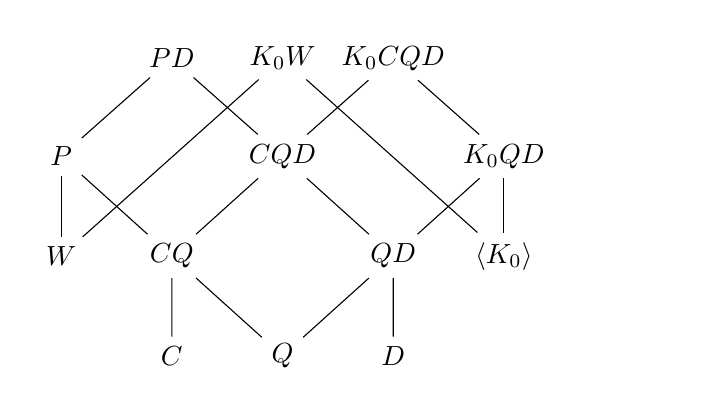
\begin{tikzpicture}[every node/.style={midway}]
  \matrix[column sep={4em,between origins}, row sep={2em}] at (0,0) {
   & \node(PD) {$PD$}; & \node(KW) {$K_0W$}; &\node(KCD) {$K_0CQD$}; & \\
    \node(P) {$P$}; && \node(CQD) {$CQD$}; && \node(KD) {$K_0QD$}; \\
     \node(W) {$W$}; & \node(CQ) {$CQ$}; && \node(QD) {$QD$}; &\node(K0) {$\gen{K_0}$}; & \\
   & \node(C) {$C$}; & \node(Q) {$Q$}; & \node(D) {$D$}; && \\
  };

  \draw (W) -- (P);
  \draw (K0) -- (KD);
  \draw (K0) -- (KW);
  \draw (W) -- (KW);
  \draw (C) -- (CQ) -- (P) -- (PD);
  \draw (D) -- (QD) -- (KD) -- (KCD);
  \draw (Q) -- (CQ) -- (CQD) -- (KCD);
  \draw (Q) -- (QD) -- (CQD) -- (PD);

\end{tikzpicture}
\end{figure}
% ......................................................................

\end{frame}

\begin{frame}[fragile]{A Corollary --- revisited}
The the group of $3$-qubit Clifford+$\CS$ operators is an amalgamated product of
three finite groups: 
\[
\begin{tikzcd}[ampersand replacement=\&]
  \&\& W\arrow[dd]\arrow[dr] \\
  \& CQD\arrow[rr] \arrow[dd]
  \&\& PD\arrow[dd, dashed]
  \\
  \gen{K_0} \arrow[rr]\arrow[dr]
  \&\& K_0W\arrow[dr, dashed]\\
  \& K_0CQD\arrow[rr, dashed]
  \&\& \CliffordCS(3)
\end{tikzcd}
\]

\end{frame}
\subsection{Proof outline for the theorem about $U_n(\di)$}
\begin{frame}[fragile]{Proof outline for the theorem about $U_n(\di)$}
  \begin{itemize}
  \item Amy et al. gave an exact synthesis algorithm in
    \cite{Amy-Glaudell-Ross}, which for $e \in U_n(\di)$, outputs an
    unique word $normal(e)$ in one- and two-level matrices.
  \item We show $e$ is $\Delta$-related to $normal(e)$, which is
    implied by the following.
  \item For any elements $s$ and $r$ and generator $G$ such that
    $s=rG$, $normal(s)$ is $\Delta$-related to $normal(r)G$. In
    picture,
    
    \begin{minipage}{0.4\textwidth}
      \[
  \xymatrix@C=0.5ex@R=3ex{
    s \ar[rrrrrrrr]^<>(.5){G}\ar@{=>}[dr]_<>(.4){N_1} &&&&&&&& r\ar@{=>}[dl]^<>(.4){N'_1}\\
    &{}\ar@{=>}[dr]_<>(.4){N_2}\ar@{}[rrrrrr]|<>(.5){\displaystyle\simr}&&&&&&{}\ar@{=>}[dl]^<>(.4){N'_2}\\
    &&{}\ar@{=>}[dr]_<>(.4){\cdots}&&&&{}\ar@{=>}[dl]^<>(.4){\cdots}\\
    &&&{}\ar@{=>}[dr]_<>(.4){N_m}&&{}\ar@{=>}[dl]^<>(.4){N'_{m'}}\\
    &&&&I \\
  }
\] \end{minipage} $\implies$ \begin{minipage}{0.4\textwidth}
\[
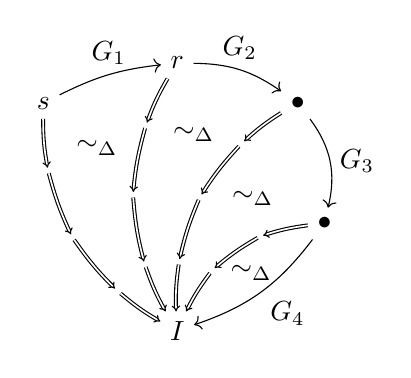
\begin{tikzpicture}[scale=1.7]
  \tikzset{inner node/.style={inner sep=0,outer sep=0.5}}
  \node(s0) at (-1,1.7) {$s$};
  \node(s1) at (0,2) {$r$};
  \node(s2) at (0.9,1.7) {$\bullet$};
  \node(s3) at (1.1,0.8) {$\bullet$};
  \node(I) at (0,0) {$I$};
  \draw [->] (s0) edge[bend left=10] node[above] {$G_1$} (s1);
  \draw [->] (s1) edge[bend left=17] node[above] {$G_2$} (s2);
  \draw [->] (s2) edge[bend left=25] node[right] {$G_3$} (s3);
  \draw [->] (s3) edge[bend left=17] node[below right] {$G_4$} (I);
  \path [inner node] (s0) edge[bend right,draw=none]
  node(s01) [pos=0.2] {}
  node(s02) [pos=0.5] {}
  node(s03) [pos=0.8] {}
  (I);
  \draw [] (s0) edge[-implies,double,bend right=5] (s01);
  \draw [->] (s01) edge[-implies,double,bend right=5] (s02);
  \draw [->] (s02) edge[-implies,double,bend right=5] (s03);
  \draw [->] (s03) edge[-implies,double,bend right=5] (I);
  \path [inner node] (s1) edge[bend right,draw=none]
  node(s11) [pos=0.2] {}
  node(s12) [pos=0.5] {}
  node(s13) [pos=0.8] {}
  (I);
  \draw [] (s1) edge[-implies,double,bend right=5] (s11);
  \draw [->] (s11) edge[-implies,double,bend right=5] (s12);
  \draw [->] (s12) edge[-implies,double,bend right=5] (s13);
  \draw [->] (s13) edge[-implies,double,bend right=5] (I);
  \path [inner node] (s2) edge[bend right,draw=none]
  node(s21) [pos=0.2] {}
  node(s22) [pos=0.5] {}
  node(s23) [pos=0.8] {}
  (I);
  \draw [] (s2) edge[-implies,double,bend right=5] (s21);
  \draw [->] (s21) edge[-implies,double,bend right=5] (s22);
  \draw [->] (s22) edge[-implies,double,bend right=5] (s23);
  \draw [->] (s23) edge[-implies,double,bend right=5] (I);
  \path [inner node] (s3) edge[bend right,draw=none]
  node(s31) [pos=0.3] {}
  node(s32) [pos=0.7] {}
  (I);
  \draw [] (s3) edge[-implies,double,bend right=5] (s31);
  \draw [->] (s31) edge[-implies,double,bend right=5] (s32);
  \draw [->] (s32) edge[-implies,double,bend right=5] (I);
  \path (s01) --node[pos=0.5] {$\simr$} (s11);
  \path (s11) --node[pos=0.5] {$\simr$} (s21);
  \path (s21) --node[pos=0.6] {$\simr$} (s31);
  \path (s3) --node[pos=0.45,xshift=-2] {$\simr$} (I);
\end{tikzpicture}
\]
\end{minipage}
  \end{itemize}
\end{frame}



\begin{frame}[fragile]{Proof outline for the theorem about $U_n(\di)$}
  \begin{itemize}
  \item The above ``commuting triangle'' is implied by a ``commuting square'':
    
    \begin{minipage}{0.3\textwidth}
\[
    \vcenter{
      \xymatrix{
        s \ar[r]^{G}\ar@{=>}[d]_{N}\ar@{}[dr]|<>(.5){\displaystyle\simr} &
        r\ar@{=>}[d]^{\vec N'}\\
        t\ar@{->}[r]^{\vec G'} &
        q.
      }
    }
\]
 \end{minipage} $\implies$     \begin{minipage}{0.5\textwidth}
\[
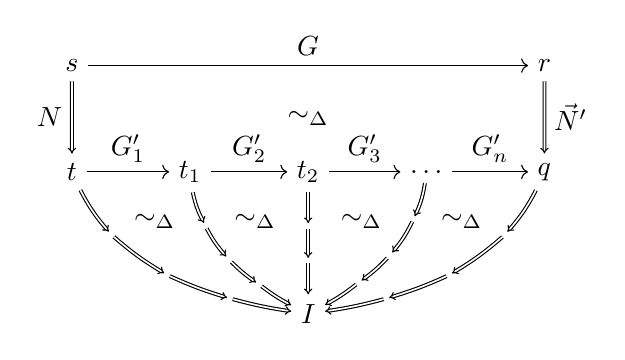
\begin{tikzpicture}[xscale=1.5,yscale=0.9]
  \tikzset{inner node/.style={inner sep=0,outer sep=0.5}}
  \node(s) at (-2,3.5) {$s$};
  \node(r) at (2,3.5) {$r$};
  \node(t) at (-2,2) {$t$};
  \node(t1) at (-1,2) {$t_1$};
  \node(t2) at (0,2) {$t_2$};
  \node(t3) at (1,2) {$\ldots$};
  \node(q) at (2,2) {$q$};
  \node(I) at (0,0) {$I$};
  \draw[->] (s) -- node[above]{$G$} (r);
  \draw[-implies,double] (s) -- node[left]{$N$} (t);
  \draw[-implies,double] (r) -- node[right]{$\vec N'$} (q);
  \draw[->] (t) -- node[above]{$G'_1$} (t1);
  \draw[->] (t1) -- node[above]{$G'_2$} (t2);
  \draw[->] (t2) -- node[above]{$G'_3$} (t3);
  \draw[->] (t3) -- node[above]{$G'_n$} (q);
  \path [inner node] (t) edge[bend right,draw=none]
  node(t01) [pos=0.25] {}
  node(t02) [pos=0.55] {}
  node(t03) [pos=0.8] {}
  (I);
  \draw [] (t) edge[-implies,double,bend right=5] (t01);
  \draw [->] (t01) edge[-implies,double,bend right=5] (t02);
  \draw [->] (t02) edge[-implies,double,bend right=5] (t03);
  \draw [->] (t03) edge[-implies,double,bend right=5] (I);
  \path [inner node] (t1) edge[bend right=20,draw=none]
  node(t11) [pos=0.25] {}
  node(t12) [pos=0.55] {}
  node(t13) [pos=0.8] {}
  (I);
  \draw [] (t1) edge[-implies,double,bend right=5] (t11);
  \draw [->] (t11) edge[-implies,double,bend right=5] (t12);
  \draw [->] (t12) edge[-implies,double,bend right=5] (t13);
  \draw [->] (t13) edge[-implies,double,bend right=5] (I);
  \path [inner node] (t2) edge[draw=none]
  node(t21) [pos=0.33] {}
  node(t23) [pos=0.67] {}
  (I);
  \draw [] (t2) edge[-implies,double] (t21);
  \draw [->] (t21) edge[-implies,double] (t23);
  \draw [->] (t23) edge[-implies,double] (I);
  \path [inner node] (t3) edge[bend left=20,draw=none]
  node(t31) [pos=0.25] {}
  node(t32) [pos=0.55] {}
  node(t33) [pos=0.8] {}
  (I);
  \draw [] (t3) edge[-implies,double,bend left=5] (t31);
  \draw [->] (t31) edge[-implies,double,bend left=5] (t32);
  \draw [->] (t32) edge[-implies,double,bend left=5] (t33);
  \draw [->] (t33) edge[-implies,double,bend left=5] (I);
  \path [inner node] (q) edge[bend left,draw=none]
  node(t41) [pos=0.25] {}
  node(t42) [pos=0.55] {}
  node(t43) [pos=0.8] {}
  (I);
  \draw [] (q) edge[-implies,double,bend left=5] (t41);
  \draw [->] (t41) edge[-implies,double,bend left=5] (t42);
  \draw [->] (t42) edge[-implies,double,bend left=5] (t43);
  \draw [->] (t43) edge[-implies,double,bend left=5] (I);
  \node at (0,2.75) {$\simr$};
  \node at (-1.3,1.3) {$\simr$};
  \node at (-0.45,1.3) {$\simr$};
  \node at (0.45,1.3) {$\simr$};
  \node at (1.3,1.3) {$\simr$};
\end{tikzpicture}
  \]
\end{minipage}

\item The commuting square depends on the pair $(N,G)$ which is finite.
\end{itemize}
\end{frame}

\section*{Future work}
%-------------------------------------------------------------------------
\begin{frame}
  \frametitle{Future work}
  \begin{itemize}
    \setlength\itemsep{1.4em}
  \item Complete relations for $4$-qubit Clifford+$\CS$ operators.
  \item Complete relations for $3$-qubit Clifford+$T$ operators.
  \item Normal forms for $3$-qubit Clifford+$\CS$ operators.
  \end{itemize}
  
\end{frame}

\begin{frame}
  \frametitle{Thank you!}
  \centering
  \huge Thank you!
\end{frame}

\begin{frame}{References}
  \scalebox{0.8}{
    \begin{minipage}{1.20\textwidth}
      \bibliographystyle{abbrv}
      \bibliography{thesis}
    \end{minipage}
  }
\end{frame}

\end{document}
